
\subsection{Analyse Amazon}
Auf der Startseite wurden wenig Fehler gefunden. Einer der häufigsten Fehler aber war auch hier fehlende Labels bei einigen Elementen. Zum Beispiel auch beim Logo, wo der Link keinen beschriebenen Text hat. Das ist ein Verstoß gegen Kriterium 4.1.2 "Name, Rolle, Wert".
\begin{figure}[H]
    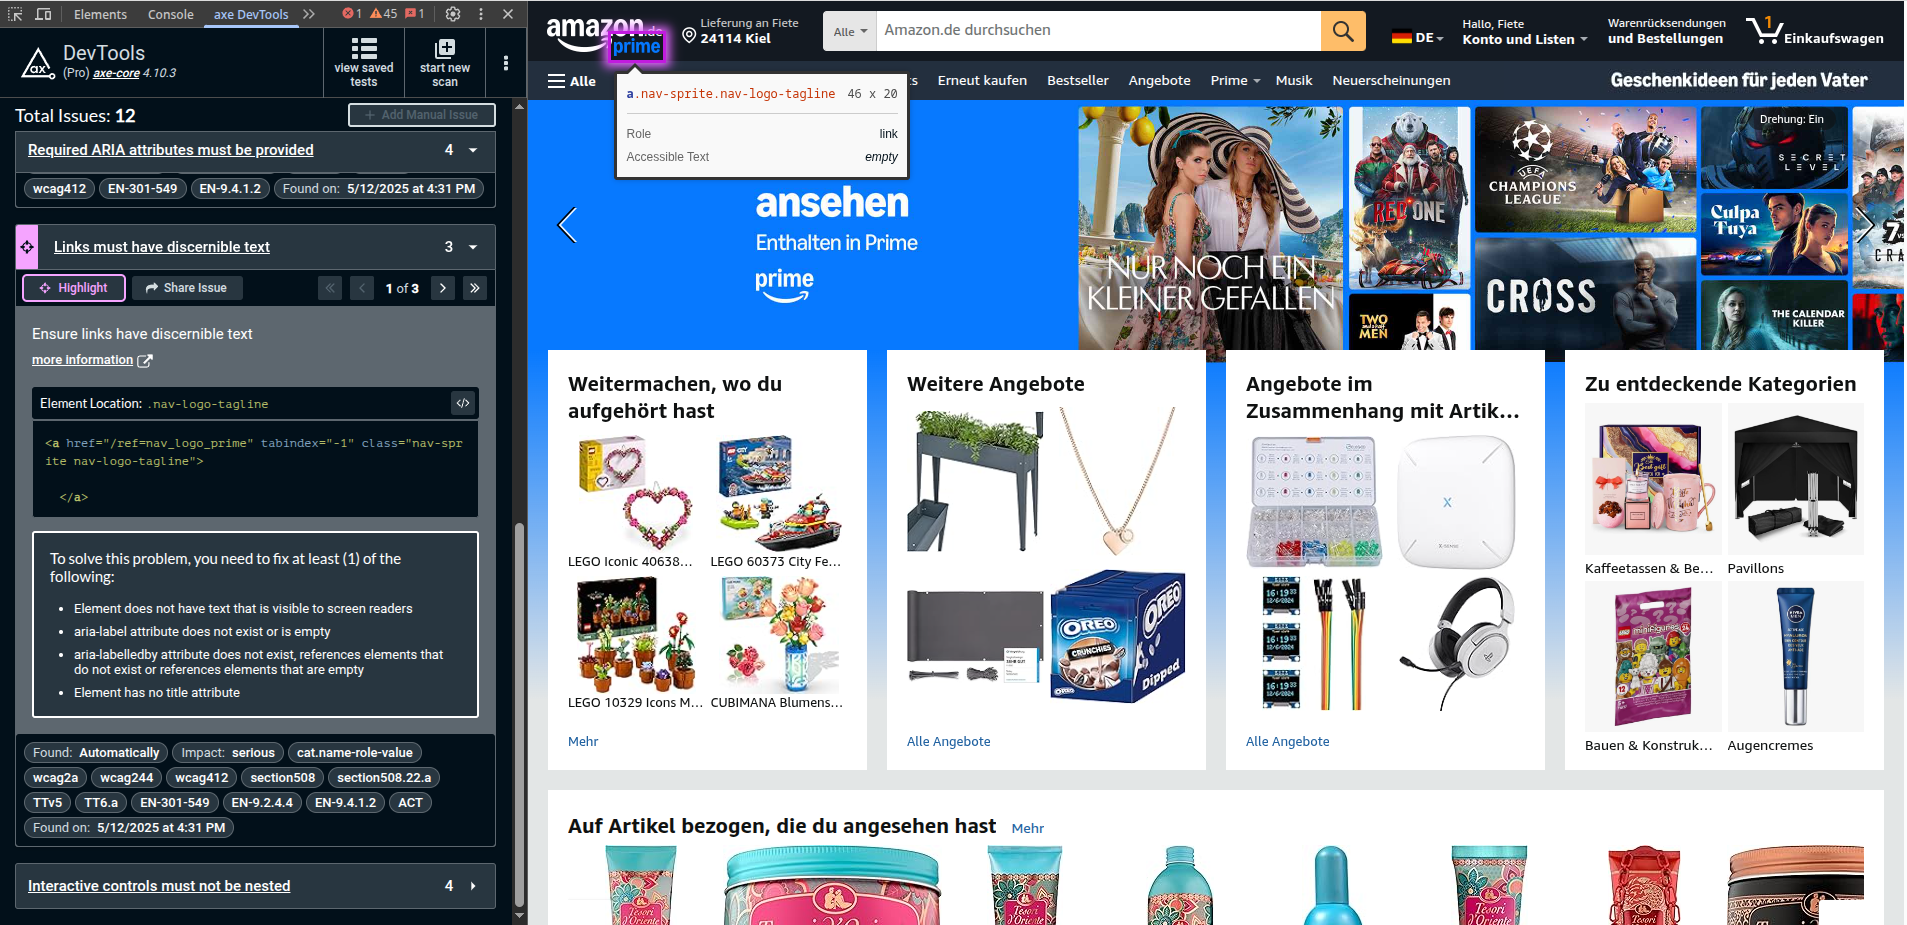
\includegraphics[width=\textwidth]{img/amazon_no-label.png}
    \caption{Fehlendes Label bei einem Link}
\end{figure}

Zusätzlich wurden noch die Produktseiten untersucht. Dabei wurde festgestellt, dass Links (Abbildung 4.31) und Buttons (Abbildung 4.32) keinen zugänglichen Namen haben. Das ist ein Verstoß gegen Kriterium 4.1.2 "Name, Rolle, Wert". Ein Button davon ist ein Bild, bei dem auch kein alternativer Text angegeben ist (Abbildung 4.33). Das ist ein Verstoß gegen Kriterium 1.1.1 "Nicht-Text-Inhalt".
\begin{figure}[H]
    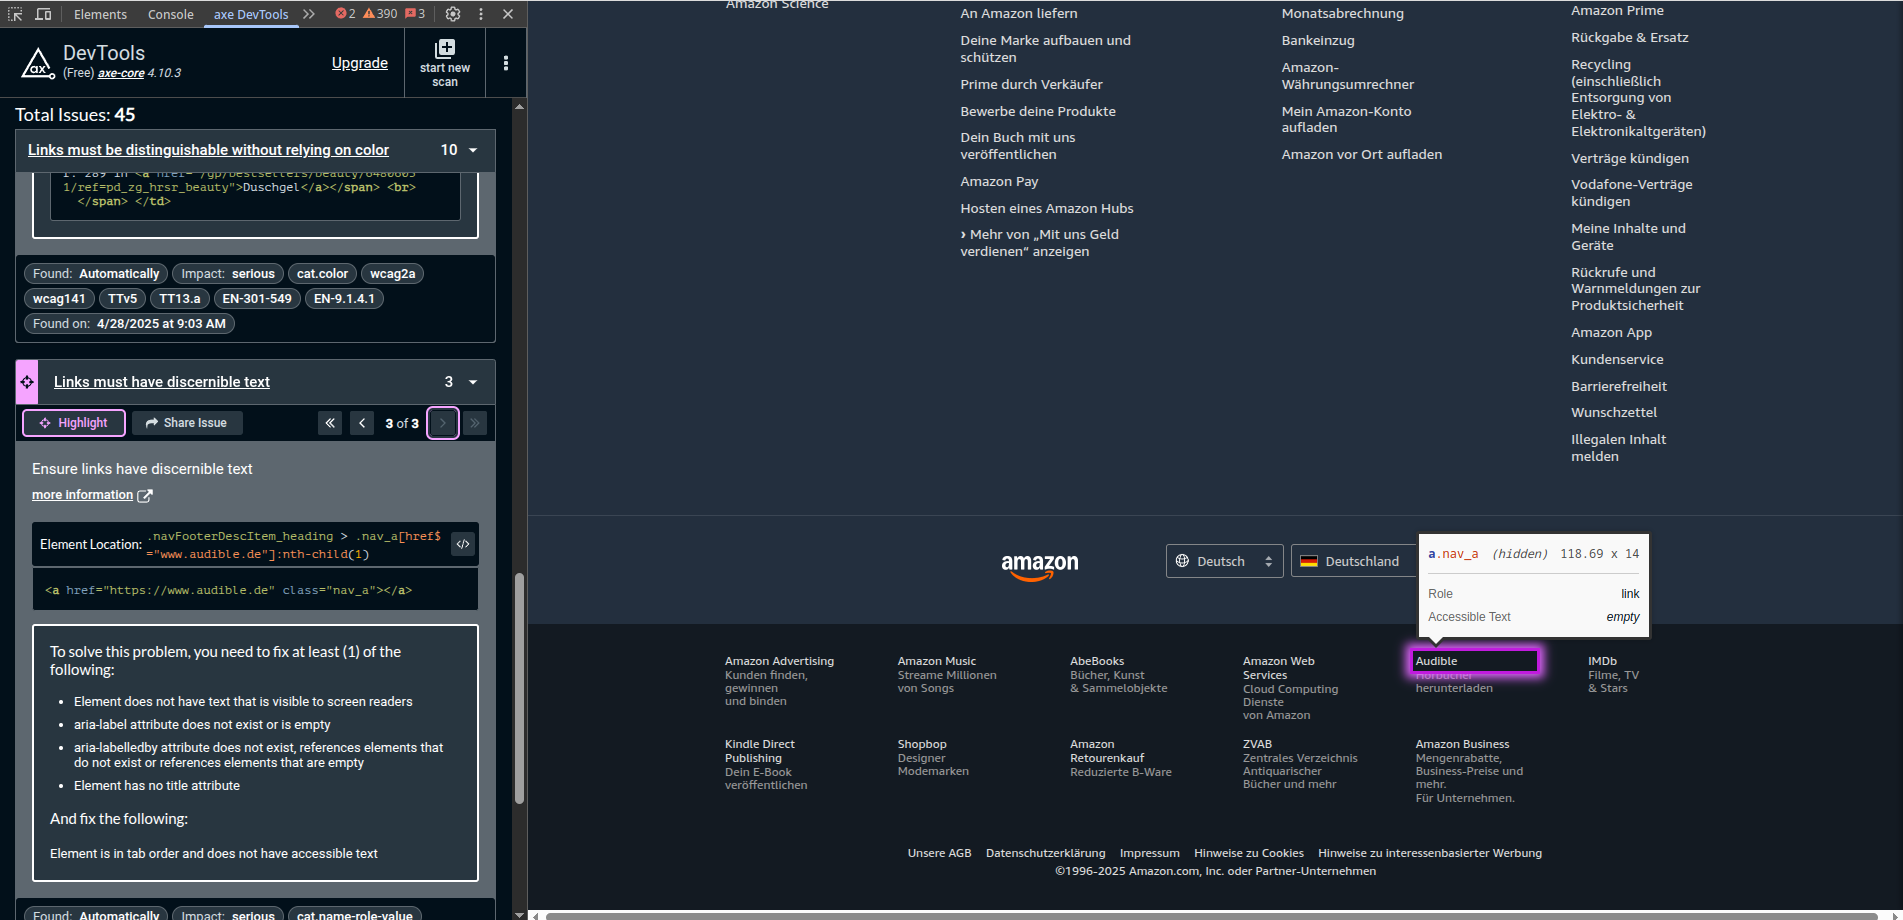
\includegraphics[width=\textwidth]{img/amazon_link-no-accessible-text.png}
    \caption{Fehlendes Label bei einem Link}
\end{figure}
\begin{figure}[H]
    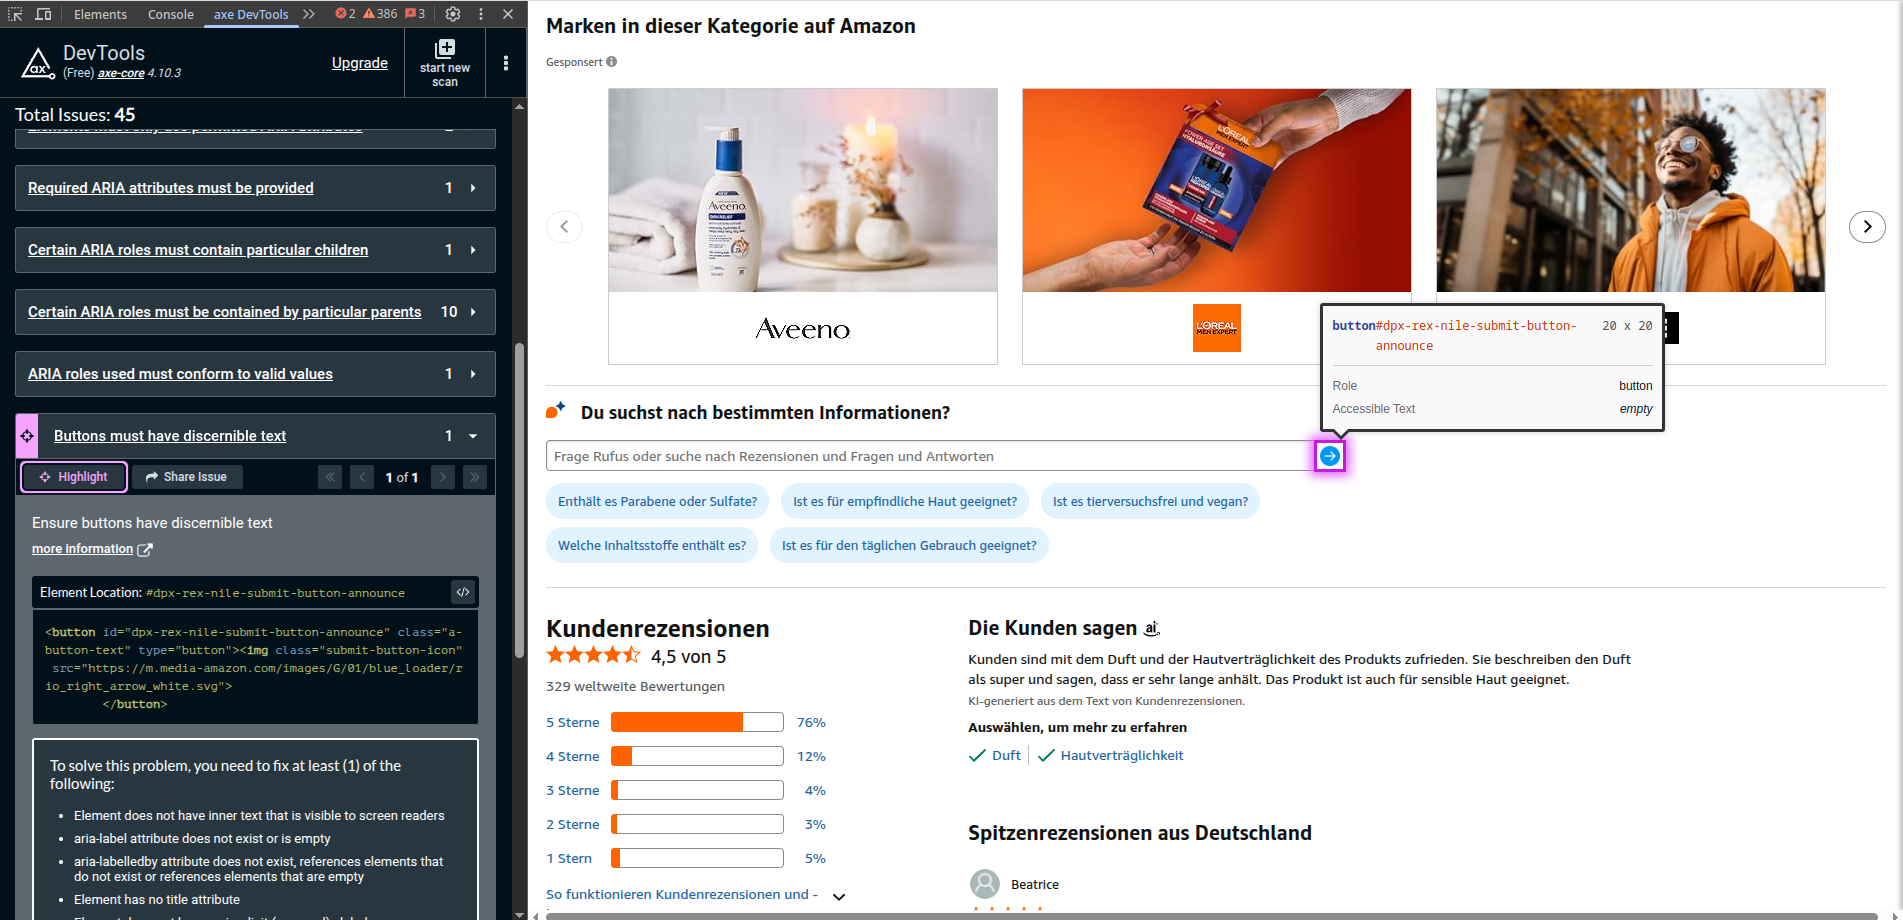
\includegraphics[width=\textwidth]{img/amazon_button-no-accessible-text.png}
    \caption{Fehlendes Label bei einem Button}
\end{figure}
\begin{figure}[H]
    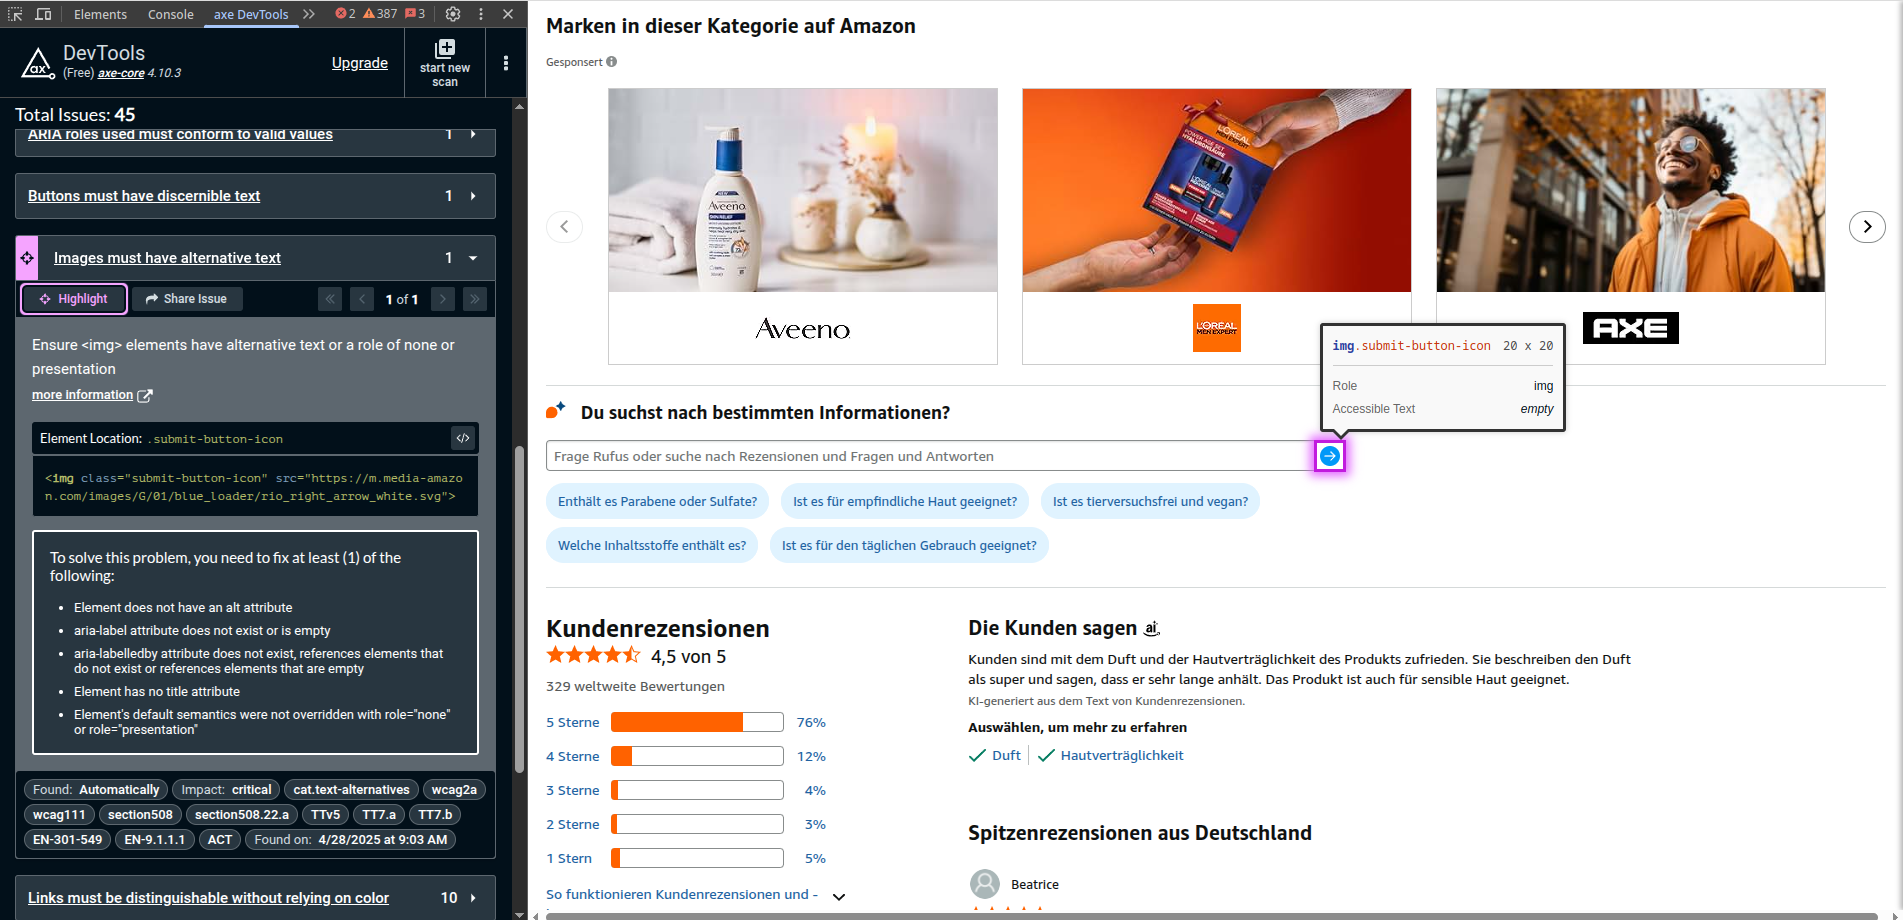
\includegraphics[width=\textwidth]{img/amazon_image-no-alt-text.png}
    \caption{Fehlender alternativer Text bei einem Bild}
\end{figure}

Die Fehler wiederholen sich natürlich auch auf den anderen Produktseiten. Auffallend ist, dass, obwohl sehr viele Bilder auf der Seite sind, nur sehr wenige Fehler bei den Bildern auftreten. Das liegt daran, dass die Bilder in der Regel mit einem alternativen Text versehen sind. Hier lässt sich auch sehr gut der Unterschied der beiden verwendeten Tools AXE und WAVE feststellen. Während AXE keine Fehler bei den alternativen Texten von Bildern feststellt, zeigt WAVE Fehler an. Grundlegend sind diese Fehler auch richtig, allerdings handelt es sich hier um die Miniaturvorschauen auf der Produktseite. Diese sind mit einem ARIA "hidden=true" ausgestattet, was bedeutet, dass diese Elemente nicht berücksichtigt werden. Damit man die Bilder trotzdem mit Screenreadern warhnehmen kann, sind alle Bilder in der großen Vorschau als Liste angelegt und nur mit CSS ausgeblendet, je nachdem welches ausgwählt ist. 

\begin{figure}[H]
    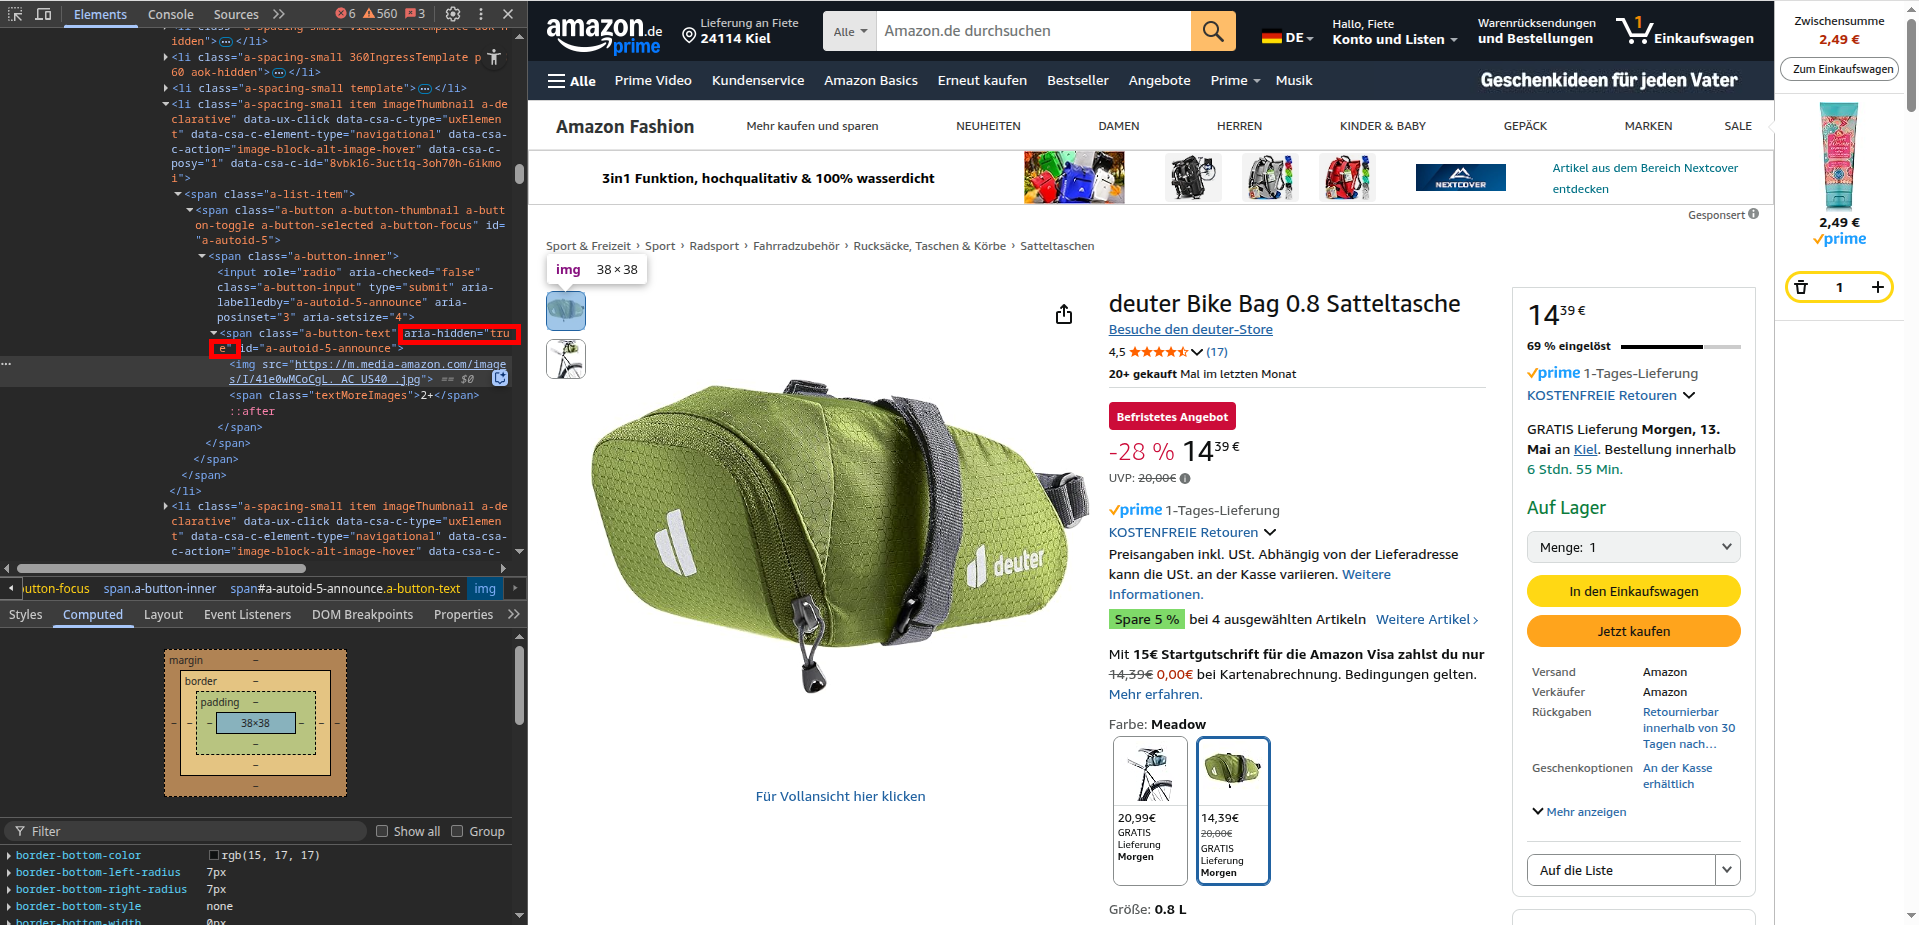
\includegraphics[width=\textwidth]{img/amazon_mini-image-no-alt-text.png}
    \caption{Vorschau Miniatur-Bild mit ARIA hidden}
\end{figure}

\begin{figure}
    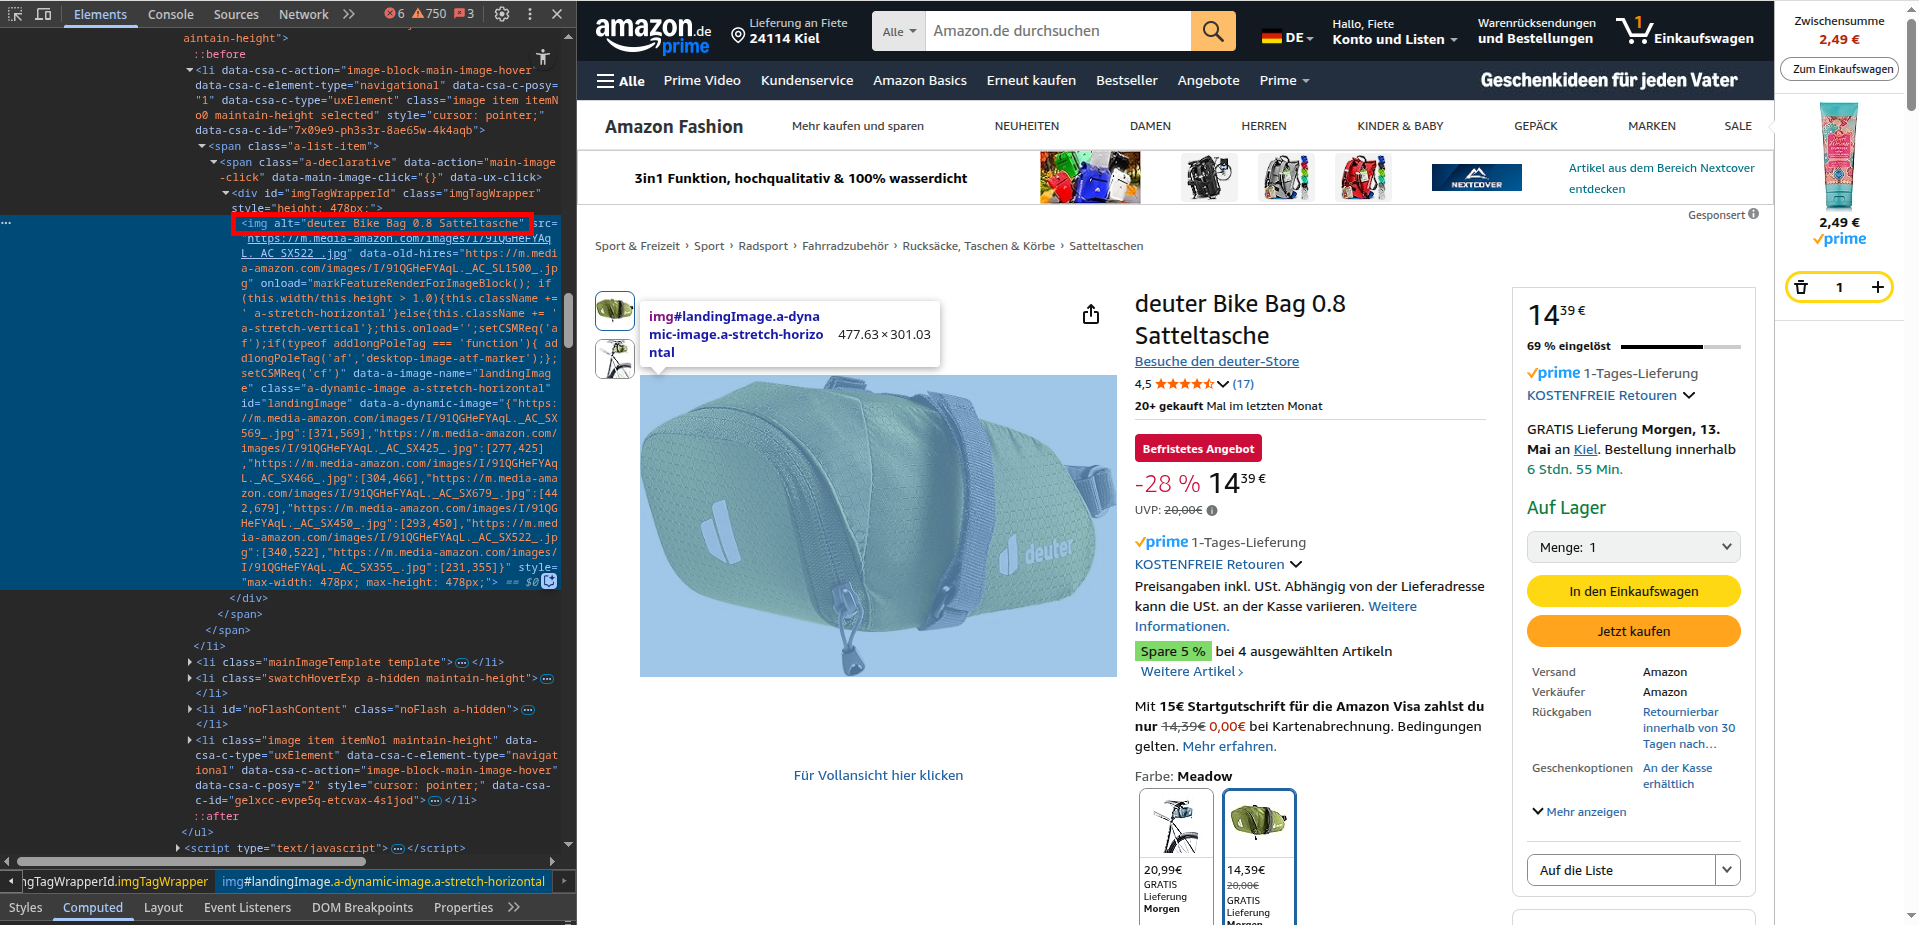
\includegraphics[width=\textwidth]{img/amazon_big-image-alt-text.png}
    \caption{Großes Vorschaubild mit alternativem Text in der Liste}
\end{figure}

In der Statistik ist der Unterschied zwischen den beiden Tools sehr gut zu erkennen. In dem Kriterium 1.1.1 \enquote{Nicht-Text-Inhalt} gibt es den größten Unterschied. In diesem Fall liegt AXE aber richtig, da der Fehler mit dem alternativen Text durch das ARIA "hidden=true" nicht mehr relevant ist.

\begin{figure}[H]
\begin{tikzpicture}
\begin{axis}[
    width=\textwidth,
    height=10cm,
    ybar,
    bar width=12pt,
    xlabel={WCAG-Kriterium},
    ylabel={Fehleranzahl},
    symbolic x coords={ 9.1.1.1, 9.1.3.1, 9.1.4.1, 9.2.4.4, 9.4.1.2 },
    xtick=data,
    x tick label style={rotate=45, anchor=east},
    ymin=0,
    ymax=300,
    enlarge x limits=0.1,
    legend style={cells={anchor=west}, legend pos=north east},
    nodes near coords,
    nodes near coords style={font=\scriptsize},
]
\addplot table[x=WCAG-Kriterium,y=Fehleranzahl_axe,col sep=tab] {csv/output/wcag_analyse_Amazon_xxxx.csv};
\addplot table[x=WCAG-Kriterium,y=Fehleranzahl_WAVE,col sep=tab] {csv/output/wcag_analyse_Amazon_xxxx.csv};
\legend{axe,WAVE}
\end{axis}
\end{tikzpicture}
\caption{Auswertung Analyse Amazon}
\end{figure}
